\documentclass{standalone}
\usepackage{tikz}
\usetikzlibrary{positioning}

\begin{document}

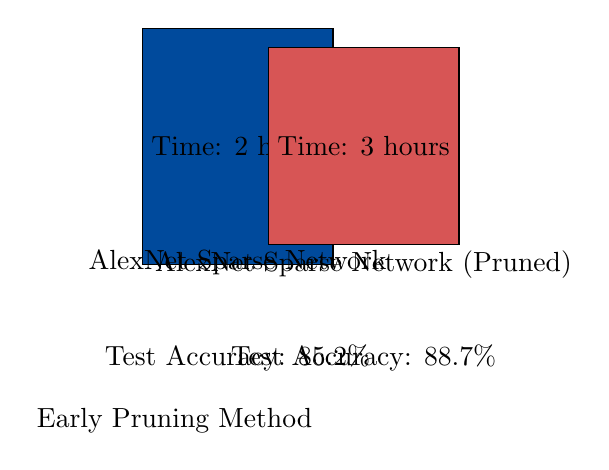
\begin{tikzpicture}[scale=0.8]
    \def\xshift{2cm} % Adjust this value to change the horizontal shift between bars

    % Define colors
    \definecolor{blue}{RGB}{0, 74, 156}
    \definecolor{red}{RGB}{215, 85, 85}

    % Nodes for the bars
    \node (bar1) at (0,0) [rectangle, draw=black, fill=blue, minimum width=2cm, minimum height=3cm] {Time: 2 hours};
    \node (bar2) at (\xshift,0) [rectangle, draw=black, fill=red, minimum width=2cm, minimum height=2.5cm] {Time: 3 hours};

    % Labels for the bars
    \node (label1) at (0,-1.5) [below] {AlexNet Sparse Network};
    \node (label2) at (\xshift,-1.5) [below] {AlexNet Sparse Network (Pruned)};

    % Test accuracies
    \node (acc1) at (0,-3) [below] {Test Accuracy: 85.2\%};
    \node (acc2) at (\xshift,-3) [below] {Test Accuracy: 88.7\%};

    % X-axis labels
    \node (xlabel1) at (-\xshift/2,-4) [below] {Early Pruning Method};
    \node (xlabel2) at (\xshift/2,-4) [below] {};
\end{tikzpicture}

\end{document}